% Подписи колонтитула
\newcommand{\colontitulAutors}{astronom\_v\_cube,~edombek}
\newcommand{\colontitulYear}{2023~}
\newcommand{\colontitulEducationalSubject}{Термодинамика и статистическая физика}
\newcommand{\colontitulTeacher}{Гавриленко В.Г.}

%Настройки шаблона
\documentclass[10pt,landscape,a4paper]{article}
\usepackage[utf8]{inputenc}
\usepackage[english, russian]{babel}
\usepackage[T1,T2A]{fontenc}  
\usepackage{upgreek} % прямые греческие ради русской традиции
\usepackage{tikz}
\usetikzlibrary{shapes,positioning,arrows,fit,calc,graphs,graphs.standard}
%\usepackage[nosf]{kpfonts}
%\usepackage[t1]{sourcesanspro}
\usepackage{multicol}
\usepackage{wrapfig}
\usepackage[top=6mm,bottom=8mm,left=4mm,right=4mm]{geometry}
\usepackage[framemethod=tikz]{mdframed}
\usepackage{microtype}
\usepackage{pdfpages}
\usepackage{amsthm,amsmath,amscd}   % Математические дополнения от AMS
\usepackage{amsfonts,amssymb}       % Математические дополнения от AMS
\usepackage{mathtools}              % Добавляет окружение multlined
\usepackage{xfrac}                  % Красивые дроби
\usepackage{physics}

\usepackage{fancyhdr} % колонтитулы

%некоторые математические команды
\newcommand{\Div}{\operatorname{div}}
\newcommand{\Grad}{\operatorname{grad}}

\let\bar\overline

\definecolor{myblue}{cmyk}{1,.72,0,.38}

\def\firstcircle{(0,0) circle (1.5cm)}
\def\secondcircle{(0:2cm) circle (1.5cm)}

\colorlet{circle edge}{myblue}
\colorlet{circle area}{myblue!5}

\tikzset{filled/.style={fill=circle area, draw=circle edge, thick},
	outline/.style={draw=circle edge, thick}}

\pgfdeclarelayer{background}
\pgfsetlayers{background,main}

%\everymath\expandafter{\the\everymath \color{myblue}}
\everydisplay\expandafter{\the\everydisplay \color{myblue}}

\renewcommand{\baselinestretch}{.8}
\pagestyle{empty}

\global\mdfdefinestyle{header}{%
	linecolor=gray,linewidth=1pt,%
	leftmargin=0mm,rightmargin=0mm,skipbelow=0mm,skipabove=0mm,
}

\makeatletter % Author: ttps://tex.stackexchange.com/questions/218587/how-to-set-one-header-for-each-page-using-multicols
\renewcommand{\section}{\@startsection{section}{1}{0mm}%
	{.2ex}%
	{.2ex}%x
	{\color{myblue}\sffamily\small\bfseries}}
\renewcommand{\subsection}{\@startsection{subsection}{1}{0mm}%
	{.2ex}%
	{.2ex}%x
	{\sffamily\bfseries}}

\makeatother
\setlength{\parindent}{0pt}

%колонтитулы
\pagestyle{fancy}
\fancyhf{}
\setlength{\headheight}{40pt}
\setlength{\headsep}{4pt}
\renewcommand{\headrulewidth}{1pt}
\fancyhead[L]{\textcopyright~\colontitulAutors}
\fancyhead[C]{Программа минимум по курсу <<\colontitulEducationalSubject>> \colontitulYear г}
\fancyhead[R]{Преподаватель:~\colontitulTeacher}

\begin{document}
	\small
	\begin{multicols*}{2}

		\section{Каноническое распределение Гиббса}
		Распределение вероятностей различных возможных состояний некоторой квазизамкнутой (некоторая часть замкнутой макроскопической системы) подсистемы. Подсистема называется квазизамкнутой, если её собственная энергия в среднем велика по сравнению с энергией её взаимодействия с остальными частями замкнутой системы (т. н. термостатами).
		$H_1(q_1,p_1)+H_2(q_2,p_2)+H_{\text{вз}}(q_1,p_1,q_2,p_2)=E=\const$ (изолированная система), \quad $H_{\text{вз}} \ll H_1, H_2$ \\
		$\rho(p,q)=\dfrac{1}{z_{\text{кл}}}\exp\left[-\dfrac{H(p,q)}{\theta}\right]$ - каноническое распределение Гиббса\\
		Каноническое распределение Гиббса обладает свойством мультипликативности: $\rho (q_1, p_1, q_2, p_2) = \rho_1(q_1, p_1) \cdot \rho_2(q_2, p_2)$. $\theta$ - модуль распределения Гиббса, определяется только средней кинетической энергией частиц термостата\\
		Из условия нормировки ($\int\rho(p,q)dpdq=1$) можем получить статистический интеграл:\\
		$z_{\text{кл}}=\int\limits_{V_{2f}}\exp\left[-\dfrac{H(p,q)}{\theta}\right]dpdq$ - зависит от свойств рассматриваемой системы\\
		
		\section{Статистическое и термодинамическое определение энтропии}
		$\divideontimes$ \textbf{Статистическое определение энтропии:} $S=k\ln(\Delta\Gamma)$, т. к. $\Delta\Gamma \geq 1 \Rightarrow S > 0$\\
		$\divideontimes$ \textbf{Термодинамическое определение энтропии:} $dS=\dfrac{\mbox{\dj}Q}{T}$ - для квазистатического процесса\\
		$k=1.38*10^{-16}$ эрг/град - постоянная Больцмана, $\Delta\Gamma$ - статистический вес состояния (число микросостояний, которые возможны в имеющимся макроскопическом состоянии)\\

		\section{Температура. Термодинамический и статистический смысл}
		Температура $\tau$ - это функция состояния, принимающая одинаковые значения для всех систем (тел), находящихся в термодинамическом равновесии, и определяемая внешними параметрами и энергией системы. Температура любой системы должна быть монотонной функцией её энергии, причем для всех частей системы эти функции должны быть либо монотонно убывающими, быть либо монотонно возрастающими.\\
		Температура является мерой средней кинетической энергии теплового движения молекул\\

		\section{Первый принцип термодинамики}
		Физически первое начало термодинамики - это уравнение баланса энергии\\
		$dU = \mbox{\dj}Q^* + \mbox{\dj}A^*$, или $dU = \mbox{\dj}Q^* - \mbox{\dj}A$\\
		$U$ - внутренняя энергия макроскопической системы. Внутренняя энергия - функция состояния, разность значений которой в двух состояниях $U_2 - U_1$ равна работе, которую надо совершить над системой при теплоизолированном переходе из первого состояния во второе: $A^*_{12} = U_2 - U_1 = Q^*_{12}$\\
		Звездочка "$*$" означает воздействие на систему извне. В отсутствие теплоизоляции работа над системой и количество полученного тепла при переходе из одного состояния в другое зависят от способа перехода. Поэтому элементарная работа над системой $\mbox{\dj}A^*$ и элементарное количество полученного тепла $\mbox{\dj}Q^*$ не являются полными дифференциалами и часто обозначаются с использованием символа $\mbox{\dj}$\\

		\section{Теплоемкость}
		Теплоемкость - это количество тепла, которое нужно передать системе для увеличения её температуры на одну единицу измерения, например, один градус. Из первого принципа термодинамики следует, что теплоёмкость зависит не только от того, насколько изменилась внутренняя энергия, но и от того, какую работу совершила система, то есть от процесса, при котором происходит нагревание.\\
		$C = \dfrac{\mbox{\dj} Q^*}{dT}$\\
		Термостат — тело с настолько большой теплоёмкостью ($C \rightarrow \infty$), что его температура при теплообмене с какой-либо системой не изменяется.\\
		\textit{Доп.прим.}\\
		Из I закона т/д: $C_p = C_v + \left[\left(\dfrac{\partial U}{\partial V}\right)_T + p\right]\left(\dfrac{\partial V}{\partial T}\right)_p$\\
		Для идеального газа: $\left(\dfrac{\partial U}{\partial V}\right)_T = 0 \Rightarrow C_p = C_v + R$\\
		Политропический процесс: $pV^\gamma = const$ - для идеального газа, где $\gamma = \dfrac{C_p - C}{C_v - C}$\\

		\section{Второй принцип термодинамики}
		Существуют различные варианты его формулировки, вытекающие один из другого.\\
		1. Нельзя построить циклически работающий двигатель, переносящий тепло от холодного тела к горячему, без превращения механической энергии во внутреннюю (невозможно создать идеальную холодильную машину). Это эквивалентно утверждению о том, что невозможна самопроизвольная передача тепла от холодного тела к горячему.\\
		2. Нельзя построить циклически работающий двигатель, единственным действием которого является полное превращение тепла от резервуара в механическую работу (невозможно создать вечный двигатель второго рода).\\
		3. Существуют адиабатически (теплоизоизолированно) недостижимые состояния.\\
		Все эти формулировки говорят о существовании для макроскопических систем необратимых процессов, которые могут протекать только в одном направлении. Действительно, вполне возможна самопроизвольная передача тепла от горячего тела к холодному, но не наоборот. Вполне возможно полное превращение механической работы в тепло (например, за счёт трения), но обратный процесс неосуществим.\\
		4. $\dfrac{\mbox{\dj} Q^*}{T} = dS$\\

		\section{Цикл Карно}
		Цикл Карно — это идеальный термодинамический цикл. Тепловая машина, работающая по этому принципу, обладает максимальным КПД. Цикл Карно является обратимым: он может быть проведен как в прямом, так и в обратном направлении, при этом энтропия адиабатически изолированной системы не меняется.\\
		\begin{tabular}{cc}
			\multirow{5}{*}{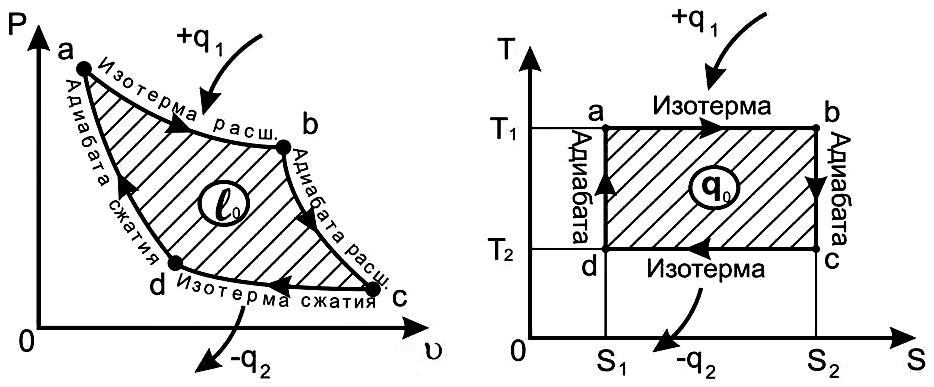
\includegraphics[width=0.55\linewidth]{td_imgs/karno_1}} & $\divideontimes$ $a \rightarrow b$ - изотермическое расширение\\
			{} & $\divideontimes$ $b \rightarrow c$ - адиабатическое расширение\\
			{} & $\divideontimes$ $c \rightarrow d$ - изотермическое сжатие\\
			{} & $\divideontimes$ $d \rightarrow a$ - адиабатическое сжатие\\\\
			{} & 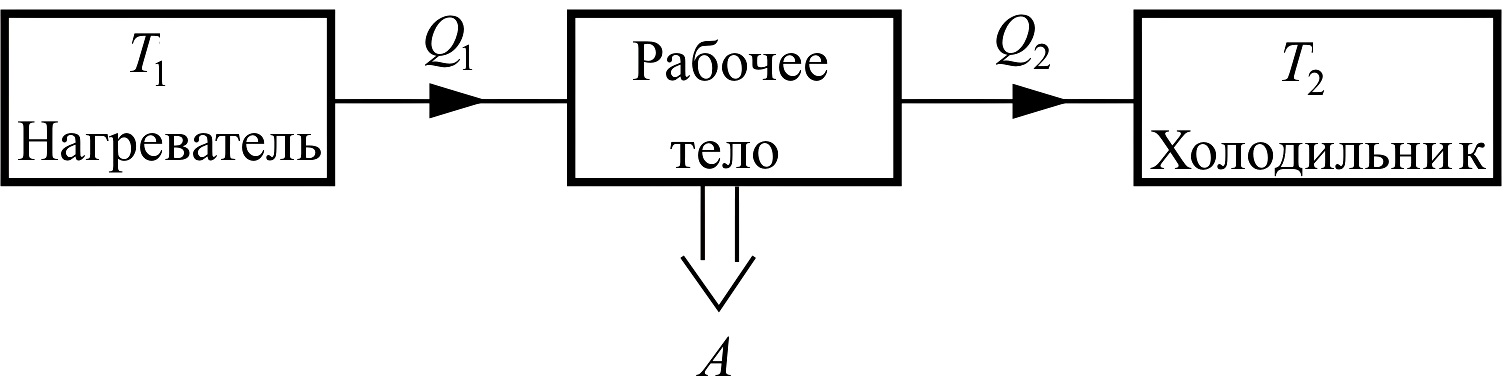
\includegraphics[width=0.35\linewidth]{td_imgs/karno_2} \\
		\end{tabular}\\\\\\
		Количество теплоты, полученное рабочим телом от нагревателя при изотермическом расширении: $Q_{\text{н}} = \int TdS = T_{\text{н}}(S_2 - S_1) = T_{\text{н}} \Delta S$\\
		Аналогично, при изотермическом сжатии: $Q_{\text{х}} = \int TdS - T_{\text{х}}(S_2 - S_1) = T_{\text{х}} \Delta S$\\
		КПД машины Карно: $\eta = \dfrac{Q_{\text{н}} - Q_{\text{х}}}{Q_{\text{н}}} = \dfrac{T_{\text{н}} - T_{\text{х}}}{T_{\text{н}}}$, т.е. КПД зависит только от температур нагревателя и холодильника. $\eta = 100\%$, только если $T_{\text{х}}$ равна абсолютному нулю (это невозможно)\\
	
		\section{Характеристические функции $F, \Phi, I$}

		Основное уравнение термодинамики: $TdS = dU + pdV$. Оно позволяет для системы в различных условиях ввести соответствующие функции состояния, называемые термодинамическими потенциалами. Это уравнение связывает 5 функций состояния: $T, S, U, p, V$. Само же состояние простой системы определяется 2 параметрами, поэтому, выбирая из 5 названных величин 2 в качестве независимых переменных, мы получаем, что основное уравнение содержит еще 3 неизвестные функции. Для их определения необходимо к основному уравнению добавить еще 2 уравнения, которыми могут быть термодинамические и калорические уравнения состояния $p = p(V, T)$ и $U = U(V, T)$, если в качестве независимых параметров выбраны в $V$ и $T$.\\\\

		$\divideontimes$ Выберем независимыми переменными $S$ и $V$:\\
		$U = U(S,V), \quad dU = TdS - pdV$\\
		$T$ и $p$ определяем как зависимые переменные: $T = \left(\dfrac{\partial U}{\partial S}\right)_V, \quad p = - \left(\dfrac{\partial U}{\partial V}\right)_S$\\
		Из двух уравнений определили зависимые переменные: $U, T, P$\\
		$U$ - характеристическая функция независимых переменных (или т/д потенциал)\\
		$TdS+SdT-SdT = dU+pdV$ - преобразование Лежандра\\
		$d(U-ST) = dF = -SdT - pdV, \quad F -$ свободная энергия, характеристическая функция для независимых переменных $T$ и $V$: $F = F(T, V)$\\
		$S = \left(\dfrac{\partial F}{\partial T}\right)_V, \quad p = - \left(\dfrac{\partial F}{\partial V}\right)_T$\\	
		$-dF = dA$ - в изотермическом процессе работа, совершаемая системой, является убылью ф-ии $F$\\
		$U = F+TS = F-T\left(\dfrac{\partial F}{\partial T}\right)_V$ - 1-ое уравнение Гиббса-Гельмгольца ($TS$ - связанная энергия)\\\\

		$\divideontimes$ Выберем независимыми переменными $T$ и $p$:\\
		$dF = -SdT - pdV - Vdp + Vdp$\\
		$d\left[F + pV\right] = d\Phi = S dT + V dp$, \quad $\Phi$ - термодинасический потенциал Гиббса, \quad $\Phi = \Phi(T, p)$\\
		$\Phi = U-ST+pV, \quad S = \left(\dfrac{\partial \Phi}{\partial T}\right)_p, \quad V = \left(\dfrac{\partial \Phi}{\partial p}\right)_T$\\
		$U = \Phi - T \left(\dfrac{\partial \Phi}{\partial T}\right)_p - p \left(\dfrac{\partial \Phi}{\partial p}\right)_T$ - 2-ое уравнение Гиббса-Гельмгольца\\\\

		$\divideontimes$ Выберем независимыми переменными $S$ и $p$:\\
		$dU = TdS - pdV - Vdp + Vdp \quad \Rightarrow \quad - pdV - Vdp = d(pV)$\\
		$d\left[U + pV\right] = dI = T dS + V dp$, \quad $I$ - тепловая функция (энтальпия), \quad $I = I(S, p)$\\
		Физический смысл энтальпии: при изобарных процессах ($p = const$) изменение энтальпии равно поглощённому количеству теплоты: $dI = dQ^*$\\
		$C_p = \left(\dfrac{\partial I}{\partial T}\right)_p, \quad T = \left(\dfrac{\partial I}{\partial S}\right)_p, \quad V = \left(\dfrac{\partial I}{\partial p}\right)_S$\\
 
		\section{Фазовые переходы первого рода}
		Фазовый переход - переход вещества из одной термодинамической фазы в другую при изменении внешних параметров\\
		Фазовые переходы первого рода: производные химического потенциала по температуре и давлению в состоянии равновесия различны для разных фаз:\\
		$\left(\dfrac{\partial \mu_1}{\partial T}\right)_{P_0} \neq \left(\dfrac{\partial \mu_2}{\partial T}\right)_{P_0}, \quad \left(\dfrac{\partial \mu_1}{\partial P}\right)_{T_0} \neq \left(\dfrac{\partial \mu_2}{\partial P}\right)_{T_0}$\\
		При $P=const$ в равновесии двух фаз их химические потенциалы одинаковы. Поэтому оно возможно только при $T = T_0$. При всех других температурах в равновесии может существовать либо одна, либо другая фаза. Так как при фиксированных $P$ и $T$ устойчиво состояние с минимальным значением термодинамического потенциала Гиббса $\Phi$ и, соответственно, с минимальным значением химического потенциала $\mu$, то при $T < T_0$ устойчива первая фаза, а при $T > T_0$ вторая.

		\section{Распределение Максвелла-Больцмана}
		$dw_{\upsilon} =\left(\dfrac{m}{2\pi kT}\right)^{3/2}\exp\left[-\dfrac{m(\upsilon^2_x + \upsilon^2_y +\upsilon^2_z)}{2kT}\right]d\upsilon_x d\upsilon_y d\upsilon_z$ - распределение Максвелла, характеризующее вероятность того, что молекула имеет данный импульс и находится в данном элементе объёма, оно справедливо и при наличии взаимодействия между частицами системы \\
		$\left\langle n(p, r)\right\rangle = N\cdot A\exp \left[-\dfrac{(p^2_x + p^2_y + p^2_z)}{2mkT} - \dfrac{u(x,y,z)}{kT}\right]$ - \textbf{распределение Максвелла - Больцмана}\\
		Здесь $\left\langle n(p, r)\right\rangle$ - cредняя плотность числа частиц в фазовом $\mu$ - пространстве, $u(x,y,z)$ - внутренняя энергия. Оно отличается тем, что кроме обобщенных импульсов учитываются обощенные координаты\\

		\section{Формула Планка для равновесного излучения}
		$\rho_\nu=\dfrac{8\pi \nu^2}{c^3}<\mathcal{E}(\nu)>=\dfrac{8\pi \nu^3 h}{c^3}\dfrac{1}{e^{h\nu/kt}-1}$ - cпектр плотности энергии равновесного излучения\\

		\section{Третье начало термодинамики}
		При стремлении температуры к абсолютному  нулю энтропия всякой равновесной системы стремится к одному и тому же для всех систем конечному значению, которое можно положить равным нулю.\\
		$\lim\limits_{T\to 0} [S(T, x_2) - S(T, x_1)] =0$, или $\lim\limits_{T\to 0} \left(\frac{\partial S}{\partial x}\right)_T = 0$\\
		$x_1, x_2$ - набор макроскопических (внешних) параметров, от которых зависит состояние системы\\
		Из третьего начала следует, что при $T\rightarrow 0K$ изотерма совпадает с адиабатой ($S = const$)\\
		\textbf{Следствия} (при $T\rightarrow 0K$):\\
		$\divideontimes$ $C_p \rightarrow 0, \quad C_v \rightarrow 0$\\
		$\divideontimes$ Термические коэффициенты расширения $\alpha$ и давления $\gamma$:\\
		$\alpha = \dfrac{1}{V_0}\left(\dfrac{\partial V}{\partial T}\right)_p \rightarrow 0$, \quad $\gamma = \dfrac{1}{p_0}\left(\dfrac{\partial p}{\partial T}\right)_V \rightarrow 0$\\
		$\divideontimes$ Недостижимость абсолютного нуля температуры\\

		\section{Распределение Бозе-Эйнштейна}
		$<N_{\vec{k}}> = \dfrac{1}{\exp\left[\dfrac{\mathcal{E}_{\vec{k}} - \mu}{kT}\right] - 1}$\\
		Этому распределению подчиняются системы частиц с целым спином - бозоны\\
		$<N_{\vec{k}}>$ - среднее число частиц в одном квантовом состоянии, характеризующимся набором квантовых чисел $\vec{k}$, $\mu$ - химический потенциал, отнесенный к одной частице, $\mathcal{E}_{\vec{k}}$ - дискретный набор собственных значений энергии\\

		\section{Распределение Ферми-Дирака}
		$<N_{\vec{k}}> = \dfrac{1}{\exp\left[\dfrac{\mathcal{E}_{\vec{k}} - \mu}{kT}\right] + 1}$\\
		Этому распределению подчиняются системы частиц с полуцелым спином - фермионы\\
		Для фермионов справедлив принцип Паули - 2 фермиона в одном квантовом состоянии находиться не могут\\

		\section{Критерий невырожденности идеального газа}
		Невырожденность - это отсутствие квантовых свойств\\
		Классический электронный газ, подчиняющийся статистике Максвелла - Больцмана, называется невырожденным электронным газом. Квантовый электронный газ, который описывается функцией распределения Ферми - Дирака (Бозе - Эйнштейна), называется вырожденным.\\
		Критерий невырожденности: $\dfrac{(2\pi \hbar)^3 N}{V(2\pi mkT)^{\frac{3}{2}}} \ll 1$ эквивалентен условию $T\gg T_{\text{выр}} = \dfrac{\hbar^2}{mk} \left(\dfrac{N}{V}\right)^{\frac{2}{3}}$\\

		\section{Энергия Ферми}
		${\mathcal{E}}_F = {\mathcal{E}}_{\text{max}} = \left(3 \pi^2\right)^{\frac{2}{3}} \dfrac{\hbar^2}{2m} \left(\dfrac{N}{V}\right)^{\frac{2}{3}}$ - граничная энергия (вырождения) Ферми газа\\
		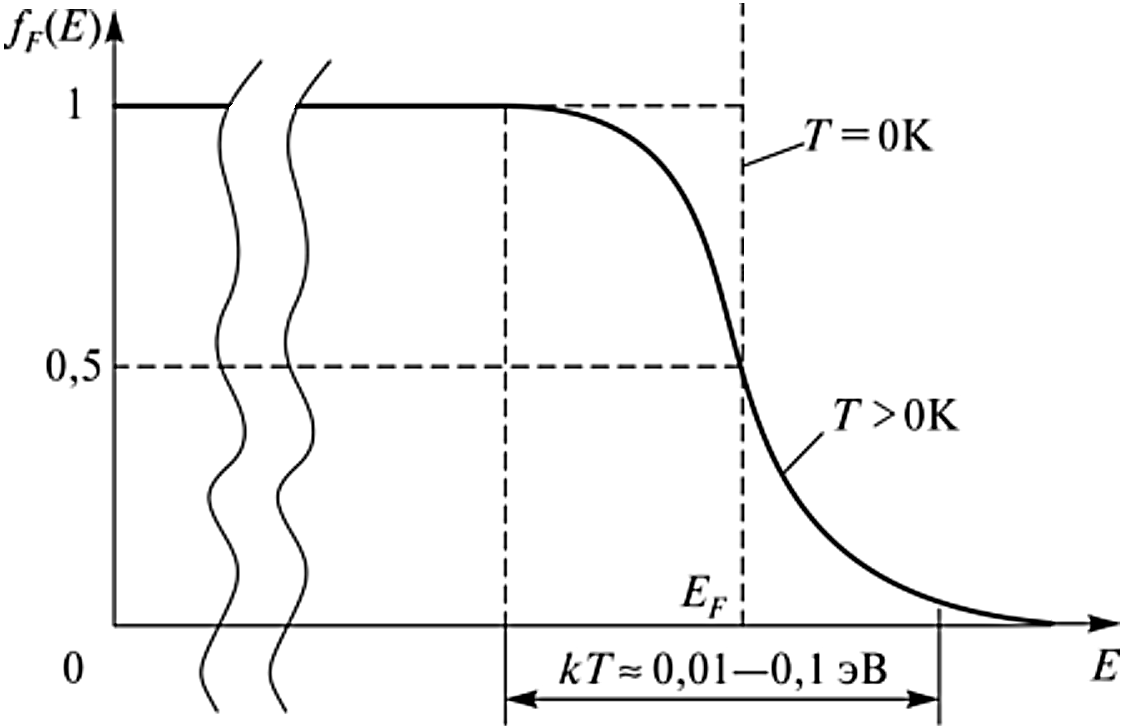
\includegraphics[width=0.4\linewidth]{td_imgs/fermi.png} \\
		Она эквивалентна химическому потенциалу системы в ее основном состоянии при абсолютном нуле температур. Энергия Ферми может также интерпретироваться как максимальная энергия фермиона в основном состоянии при абсолютном нуле температур

	\end{multicols*}
\end{document}
